\documentclass[12pt]{article}

\usepackage{sbc-template}
\usepackage[utf8]{inputenc}
\usepackage[T1]{fontenc}
\usepackage[english]{babel}
\usepackage{graphicx}
\usepackage{booktabs}
\usepackage{float}
\usepackage[hidelinks]{hyperref}

\title{Preliminary Advisor Brief: Portuguese Semantic Change in BrPoliCorpus Floor}

\author{
Jo\~ao Victor M. Corr\^ea\inst{1}
}

\address{
Interinstitutional Center for Computational Linguistics (NILC)\\
Institute of Mathematics and Computer Science\\
University of S\~ao Paulo (USP), S\~ao Carlos, SP, Brazil\\
\texttt{\footnotesize victormcorrea@usp.br}
}

\begin{document}

\maketitle

\begin{abstract}
This brief summarizes a preliminary yearly semantic-change run on Brazilian Chamber floor
speeches from 2003 to 2023. The current run covers the full corpus, trains one Word2Vec
Skip-Gram model per year, and aligns yearly spaces with Orthogonal Procrustes. The
experiment is already useful for discussion with the advisor because it shows broad coverage,
clear drift separation, and several politically relevant terms with non-trivial movement.
The main limitation is linguistic: this preliminary run used a fast lookup-only preprocessing
path, which inflated discourse markers and unstable lemmas at the very top of the ranking.
A cleaner rerun with full spaCy tagging is already in progress.
\end{abstract}

\section{Current Goal}

The immediate goal is not to claim a finished STIL result. It is to show that the new
\texttt{BrPoliCorpus floor} direction is viable, that the corpus supports a yearly diachronic
setup, and that politically meaningful vocabulary already displays measurable movement.

\section{Preliminary Setup}

\begin{itemize}
    \item Corpus: \texttt{BrPoliCorpus floor}
    \item Temporal granularity: yearly
    \item Window analyzed here: 2003--2023
    \item Method: Word2Vec Skip-Gram 300d per year + Orthogonal Procrustes alignment
    \item This run: 1 replicate, 5 epochs, full corpus coverage
    \item Main caveat: fast lookup-only preprocessing was used for this quick diagnostic run
\end{itemize}

The yearly quicklook covers 395{,}136 documents, 64.3M cleaned tokens, and 3{,}558 scored
lemmas. The unrestricted ranking is numerically strong, but the top positions are polluted by
discourse markers and noisy lemmas. That makes the run good for advisor discussion and
pipeline validation, but not yet the final paper result.

\section{What Already Looks Promising}

Figure~\ref{fig:coverage} shows that yearly coverage is strong enough to support the main
experiment. Figure~\ref{fig:curated_bar} focuses on politically interpretable terms rather
than the unrestricted top 15. Several terms already show substantial drift in the preliminary
run, including \textit{governante}, \textit{golpe}, \textit{governo}, \textit{previd\^encia},
\textit{cpi}, \textit{corrup\c{c}\~ao}, and \textit{ditadura}.

\begin{table}[H]
    \centering
    \caption{Curated political terms in the preliminary yearly run. Rank is relative to the full scored vocabulary.}
    \label{tab:curated_terms}
    \begin{tabular}{lccc}
        \toprule
        Term & Rank & Drift & Presence \\
        \midrule
        governante & 715 & 0.3527 & 1.00 \\
        golpe & 777 & 0.3476 & 1.00 \\
        governo & 1536 & 0.3121 & 1.00 \\
        previd\^encia & 2194 & 0.2869 & 1.00 \\
        cpi & 2332 & 0.2819 & 1.00 \\
        or\c{c}amento & 2592 & 0.2701 & 0.86 \\
        corrup\c{c}\~ao & 2784 & 0.2620 & 1.00 \\
        liberdade & 2883 & 0.2571 & 1.00 \\
        mil\'icia & 3024 & 0.2491 & 0.81 \\
        ditadura & 3105 & 0.2437 & 1.00 \\
        economia & 3356 & 0.2185 & 1.00 \\
        democracia & 3438 & 0.2056 & 1.00 \\
        \bottomrule
    \end{tabular}
\end{table}

Figure~\ref{fig:curated_traj} shows that the trajectory patterns for curated political terms
are not flat. They still need cleaner preprocessing and replicate checks, but they are already
sufficiently structured to justify continuing in this direction.

\section{Main Limitation of the Current Run}

The unrestricted top drift list is not yet acceptable for the paper. It is dominated by terms
such as \textit{da\'i}, \textit{ali\'as}, \textit{tampouco}, \textit{obviamente}, and by
lemmas that appear to reflect lookup errors or unstable normalization. That is consistent with
the quick diagnostic design of this run.

So the correct reading for the meeting is:

\begin{itemize}
    \item the corpus and yearly setup are viable;
    \item the pipeline is producing measurable drift and useful figures;
    \item the final candidate list should come from the clean rerun with full spaCy tagging,
    not from this quick diagnostic ranking.
\end{itemize}

\section{Next Step Already Underway}

A clean preparation pass with \texttt{pt\_core\_news\_sm} is currently running. That rerun is
the one I would trust for:

\begin{itemize}
    \item freezing the main drift candidates;
    \item running the semester robustness check;
    \item selecting terms for confirmatory BERT analysis;
    \item writing the first paper-facing Results section.
\end{itemize}

For the advisor meeting, the recommended framing is simple: the new direction is working, the
full-corpus yearly run already shows interpretable political movement, and the immediate task is
to replace the noisy quick preprocessing with the clean rerun before locking the paper claims.

\begin{figure}[H]
    \centering
    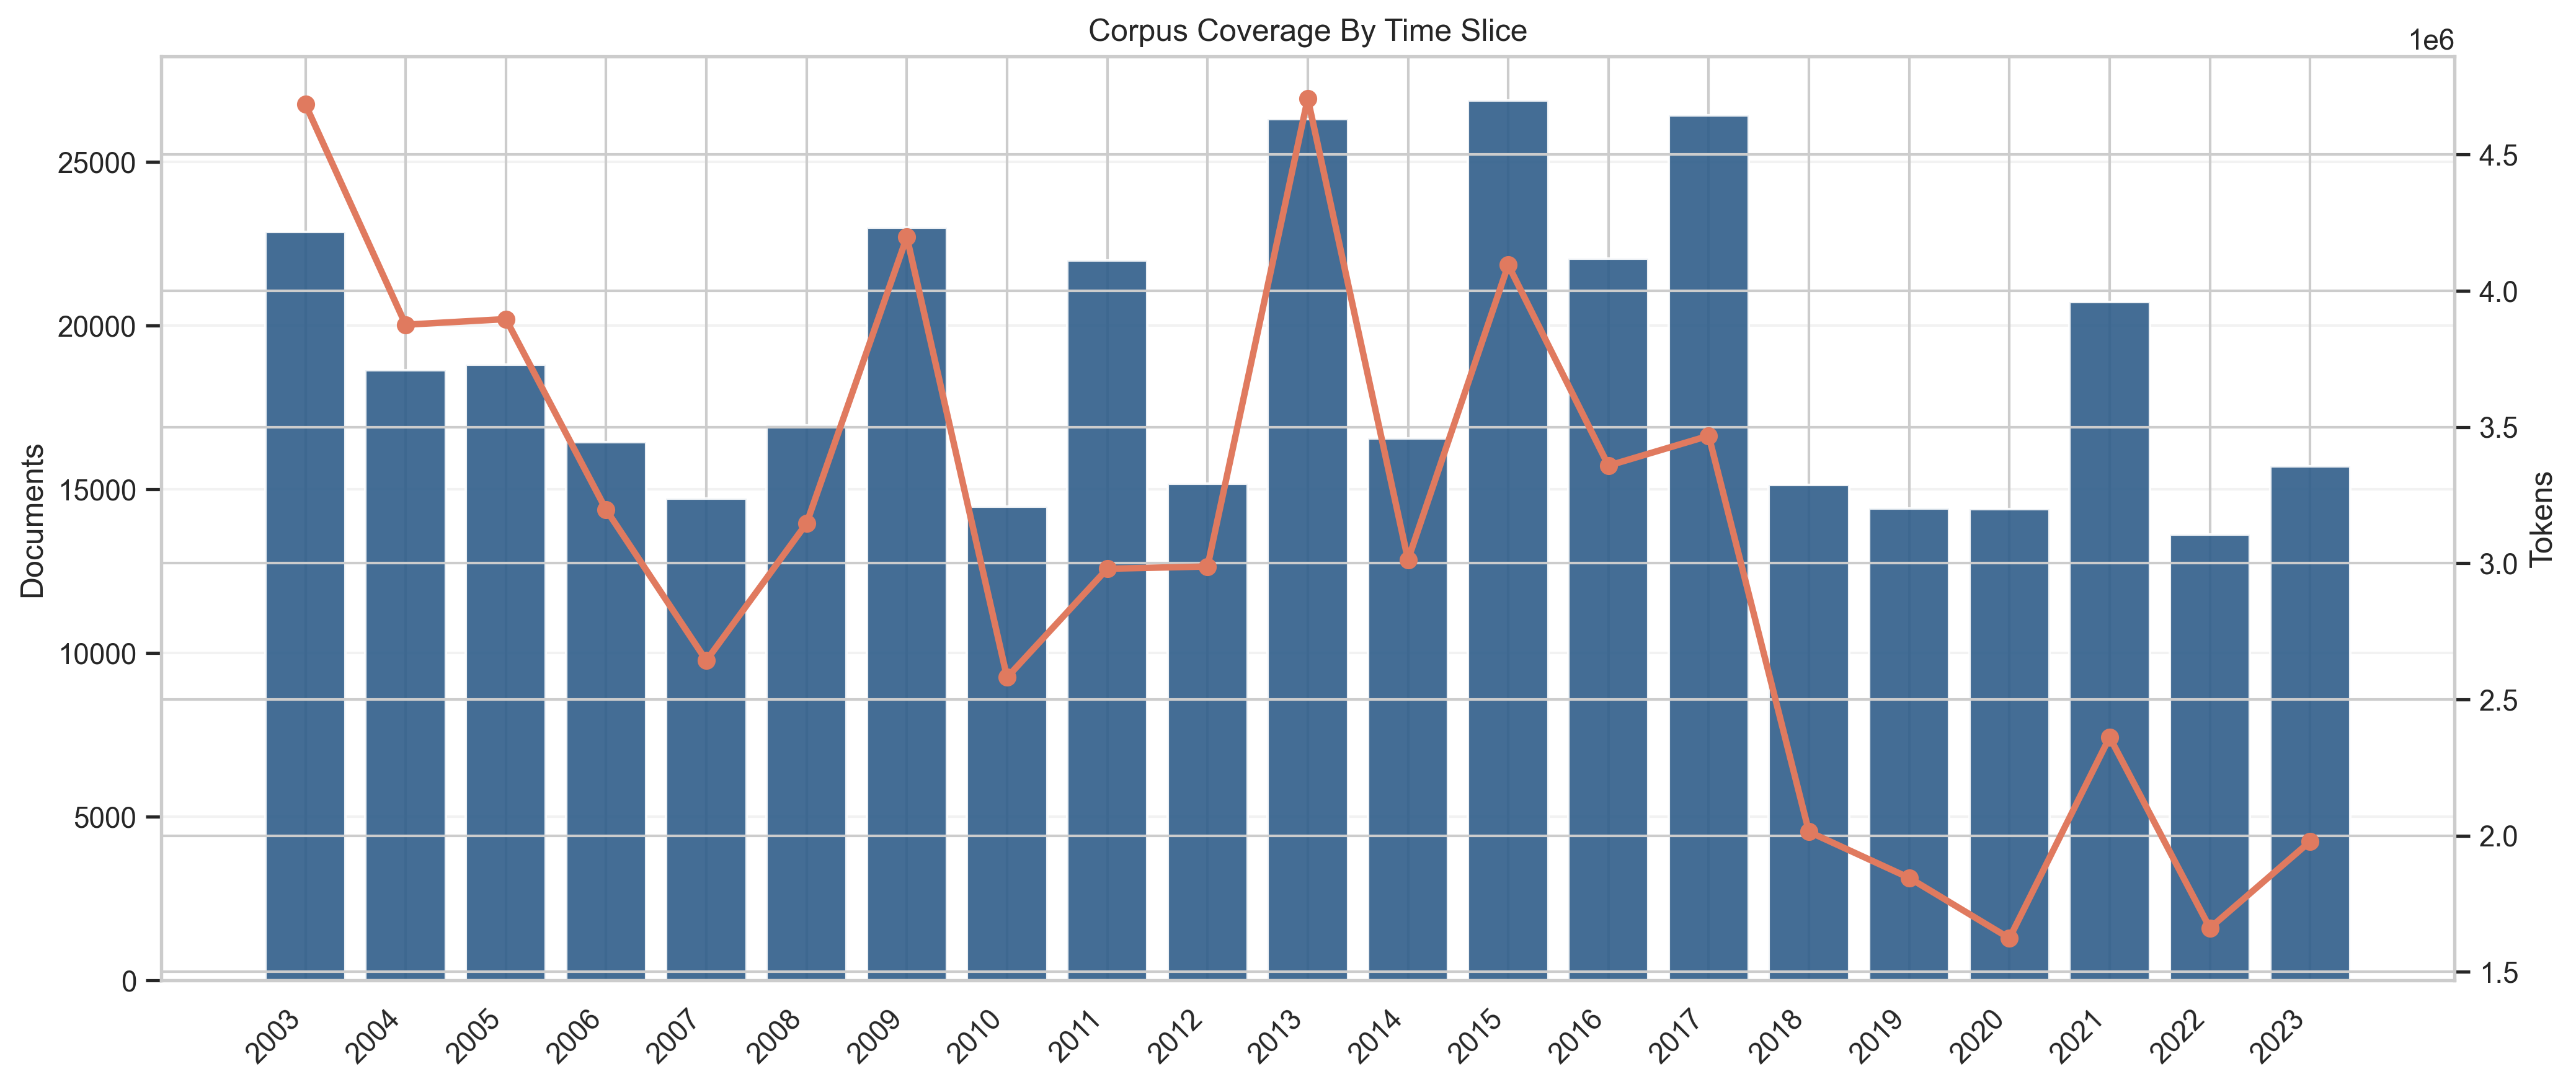
\includegraphics[width=0.82\linewidth]{figs/advisor_prelim/coverage_by_slice.png}
    \caption{Yearly document and token coverage for the preliminary 2003--2023 run.}
    \label{fig:coverage}
\end{figure}

\begin{figure}[H]
    \centering
    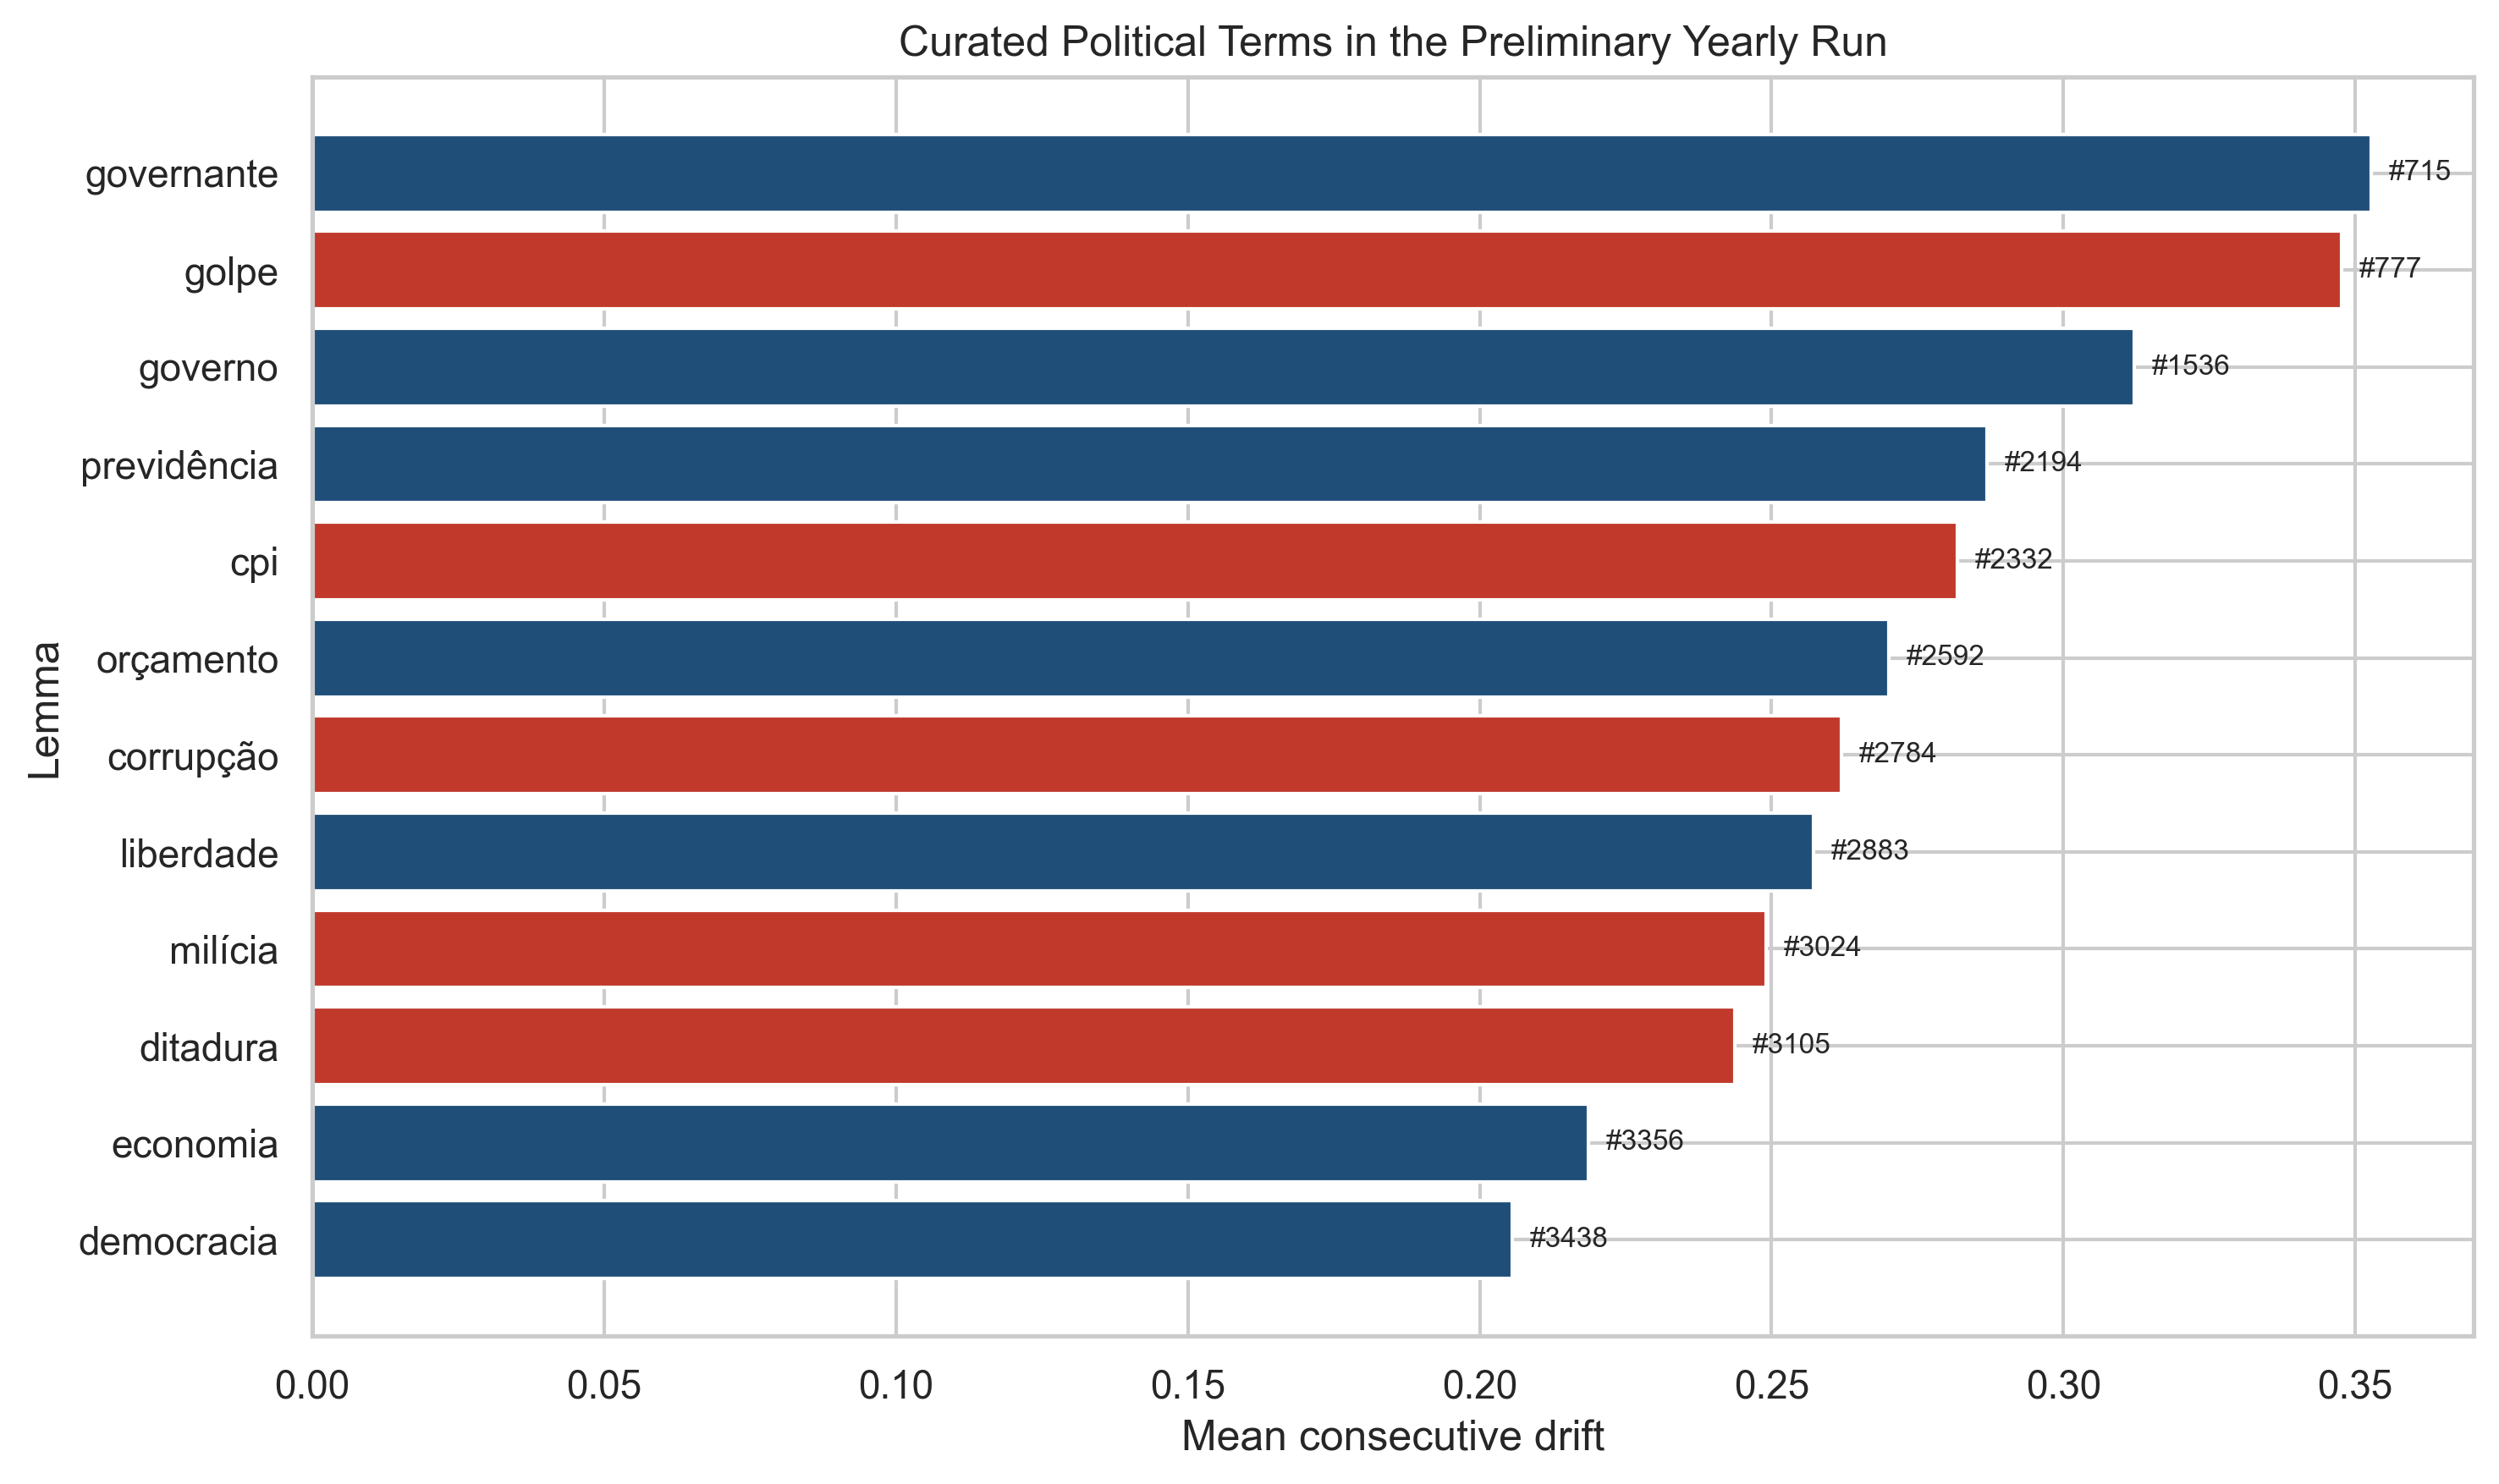
\includegraphics[width=0.82\linewidth]{figs/advisor_prelim/curated_political_terms.png}
    \caption{Curated political terms from the preliminary yearly run. The labels show each term's rank in the full vocabulary ranking.}
    \label{fig:curated_bar}
\end{figure}

\begin{figure}[H]
    \centering
    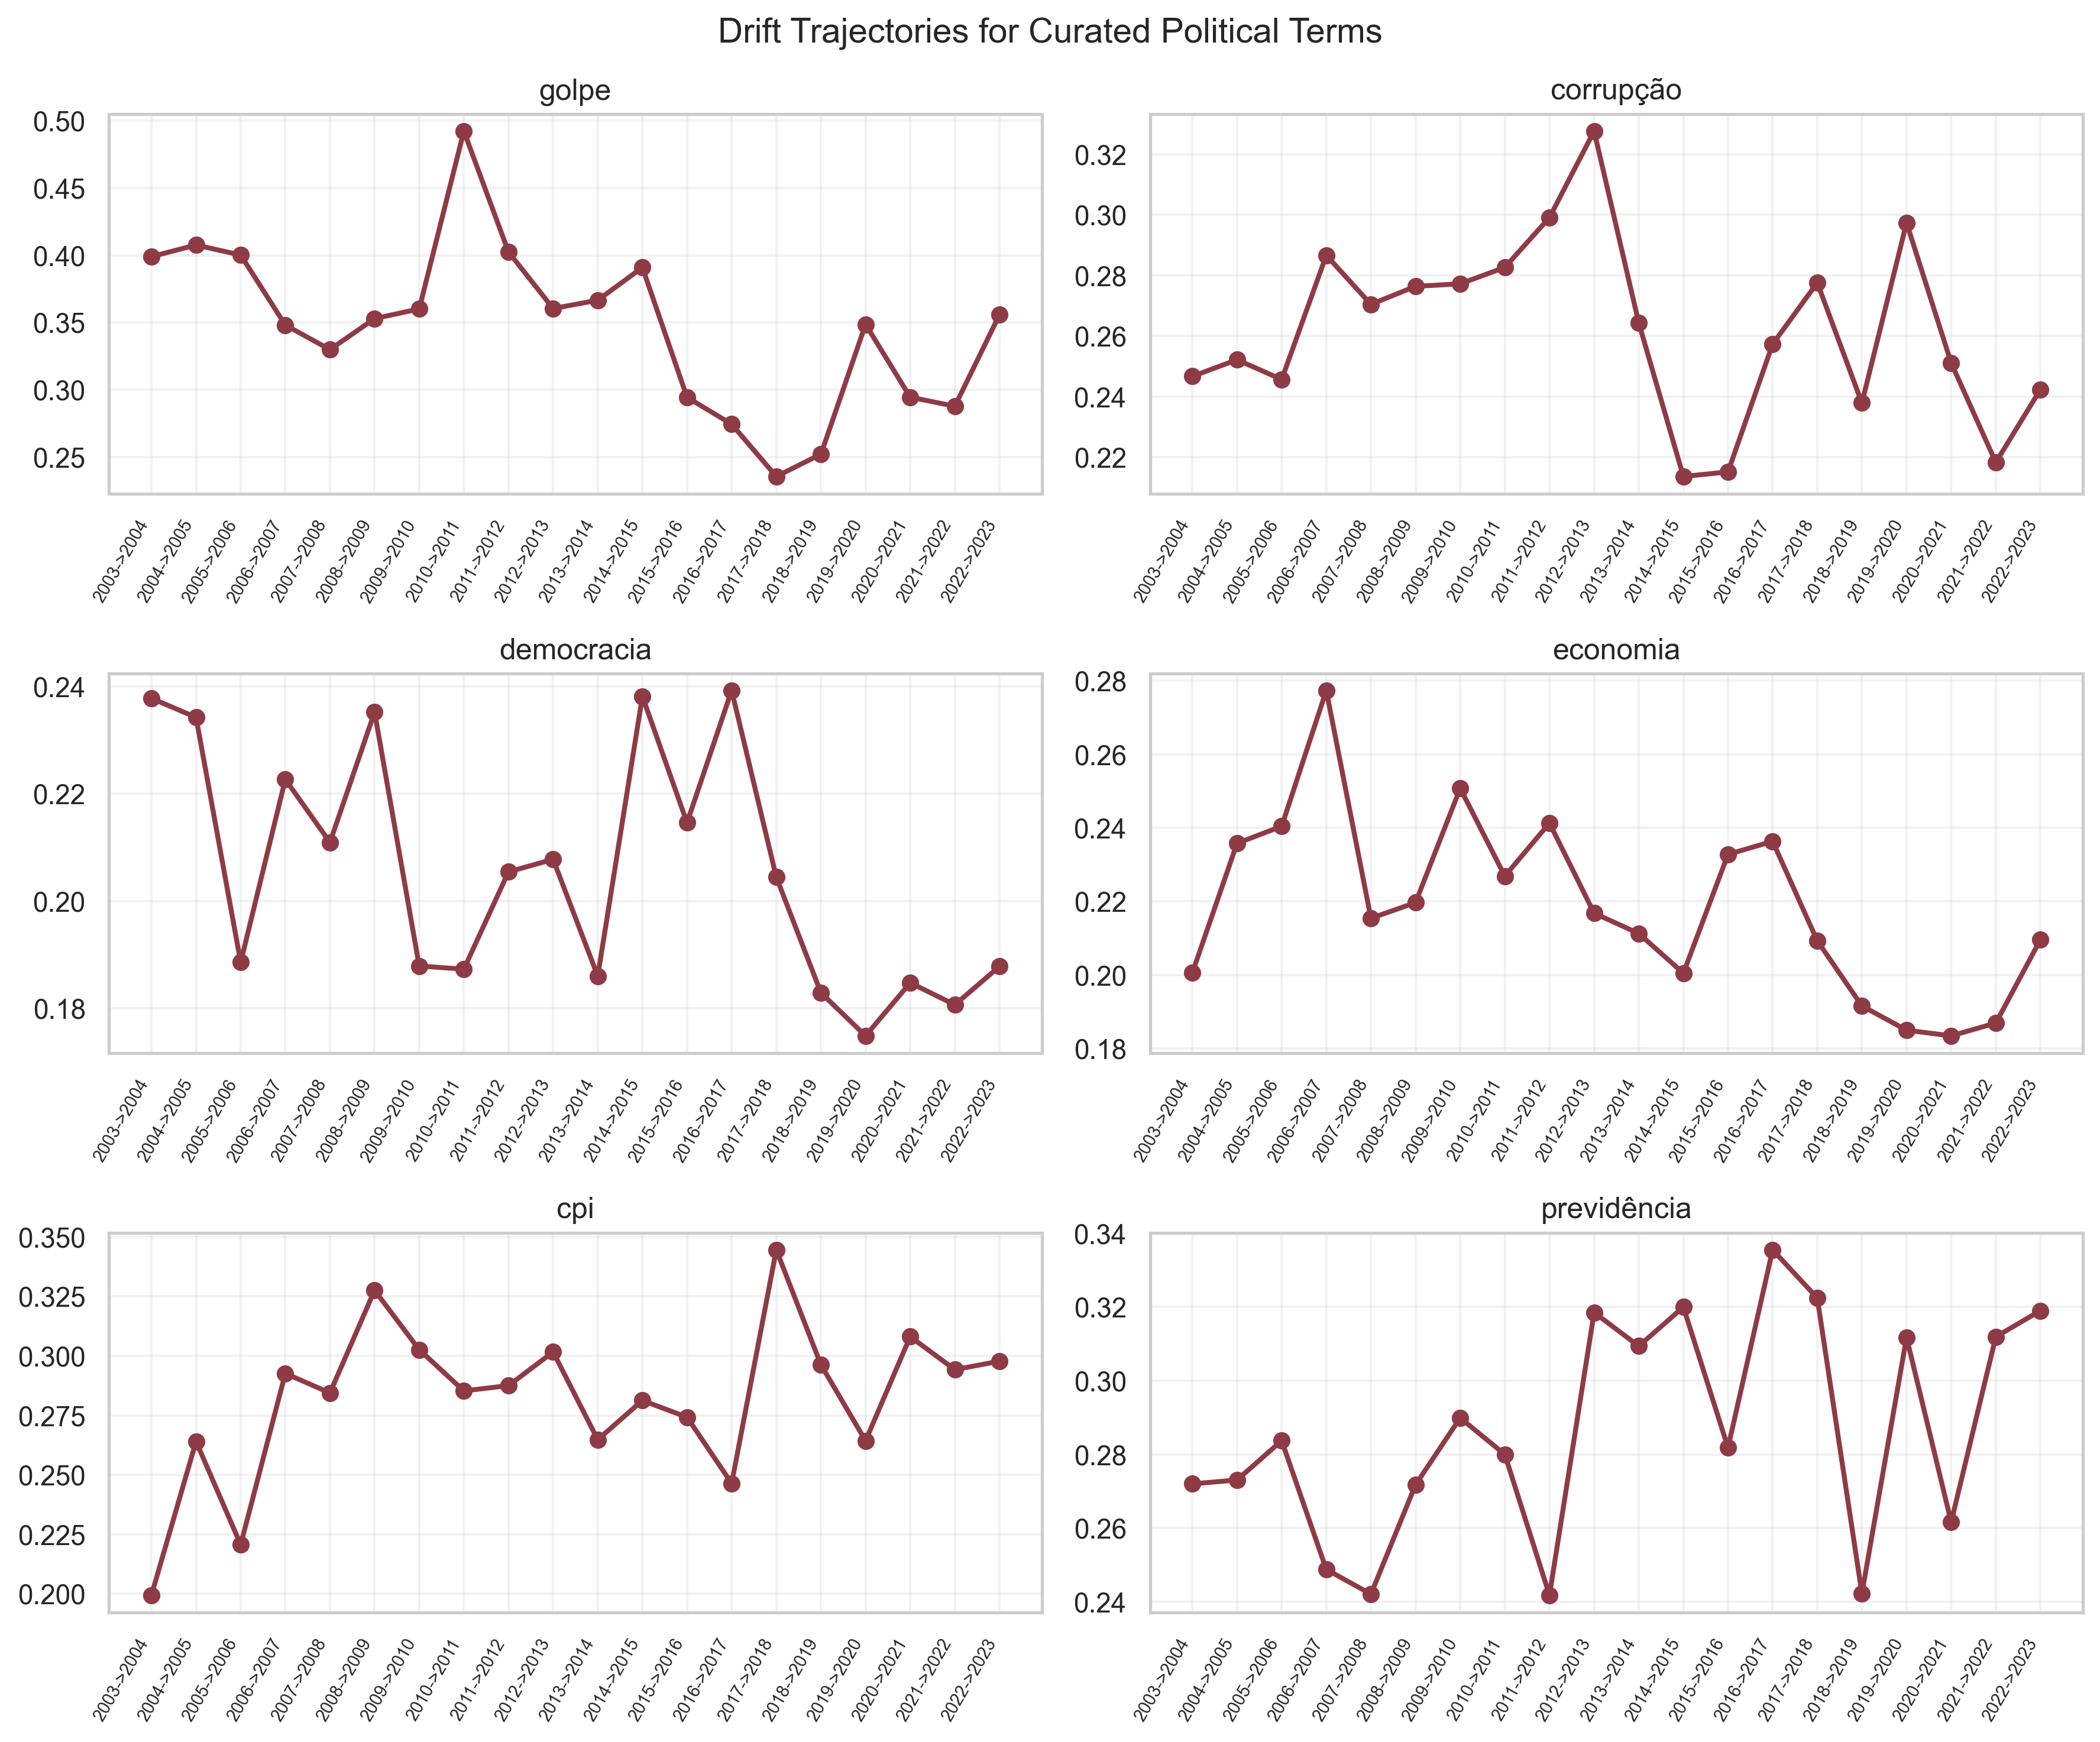
\includegraphics[width=\linewidth]{figs/advisor_prelim/curated_political_trajectories.png}
    \caption{Preliminary drift trajectories for selected political terms across consecutive yearly transitions.}
    \label{fig:curated_traj}
\end{figure}

\end{document}
